\newpage
\section {Билет 7. Распределенные запросы. Распределенные и кластерные базы данных. Распределенные транзакции.}

\begin{center}
	\textit{\underline{Распределённые запросы}}
\end{center}

Мы можем использовать сервер баз данных, чтобы запрашивать и обновлять несколько баз данных на нескольких серверах одного и того же экземпляра. Запросы такого типа называются \textbf{распределенными запросами}. Этот термин не ограничивается операторами SELECT и часто используется для более общего обозначения любой операции \hyperlink{DML_label}{DML} (Data Manipulation Language) или выполнения подпрограммы, которая возвращает объекты или ссылается на объекты вне локальной базы данных.
В распределенных запросах для разных серверов серверы баз данных могут находиться на одном хост-компьютере, в одной и той же сети или на шлюзе.

\begin{center}
	\textit{\underline{Распределённые и кластерные базы данных}}
\end{center}

\textbf{Распределённая база данных} - это такая база данных, составные части которой размещаются в различных узлах компьютерной сети в соответствии с каким-либо критерием.

Распределённая база данных — это именно единая база данных, а не произвольный набор файлов, индивидуально хранимых на разных узлах сети и являющейся распределенной файловой системой. Данные представляют собой РБД, только если они связаны в соответствии с некоторым структурным формализмом, реляционной моделью, а доступ к ним обеспечивается единым высокоуровневым интерфейсом.

Распределённые базы могут иметь разный уровень реплицированности — от полного отсутствия дублирования информации, до полного дублирования всей информации во всех распределённых копиях (например, блокчейн).

Распределение (включая фрагментацию и репликацию) базы данных по множеству узлов невидимо для пользователей. Это свойство называется прозрачностью, а технология распределения и реплицирования данных по множеству компьютеров, связанных сетью, является основополагающей для реализации концепции независимости данных от среды хранения. Это обеспечивается за счёт нескольких видов прозрачности:

\begin{enumerate}
	\item[\textbullet] прозрачность сети, а следовательно, прозрачность распределения
	\item[\textbullet] прозрачность репликации
	\item[\textbullet] прозрачность фрагментации
	\item[\textbullet] прозрачность доступа, означающая, что пользователи имеют дело с единым логическим образом базы данных и осуществляют доступ к распределенным данным точно так же, как если бы они хранились централизованно.
\end{enumerate}

В идеале полная прозрачность подразумевает наличие языка запросов к распределённой СУБД, не отличающегося от языка для централизованной СУБД.

\bigskip
Основными структурами построения кластерных баз данных являются:
\begin{enumerate}
	\item \textbf{Shared Disk (SD)} - случай, когда база данных, располагающаяся на нескольких компьютерах, использует одни и те же устройства хранения.
	
	\item \textbf{Shared Memory (SM)} - случай, когда много процессоров в базе данных, возможно, расположенных на разных машинах, используют общую (разделяемую) память.
	
	\item \textbf{Shared Nothing (SN)} - случай, когда ни устройства хранения, ни память систем не разделяются. В таких системах каждый узел обслуживает свой фрагмент базы данных, уникальность которого обеспечивается либо организацией базы данных, либо дополнительными средствами управления и мониторинга СУБД.
	
	\item \textbf{Shared Everything (SE)} - случай симбиоза SM+SD, когда СУБД использует и общие устройства ввода-вывода, и память. К таким системам относится, например, Oracle RAC.
\end{enumerate}

\begin{figure}[h]
	\centering
	\begin{subfigure}[b]{0.2\textwidth}
		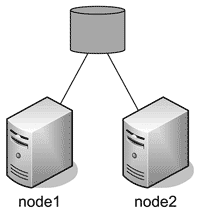
\includegraphics[width=\textwidth]{7/07_01.png}
		\caption{Shared Disk}
		\label{fig:my_label1}
	\end{subfigure}
	\hfill
	\begin{subfigure}[b]{0.2\textwidth}
		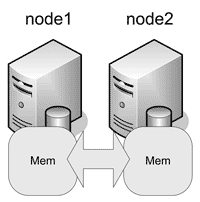
\includegraphics[width=\textwidth]{7/07_02.png}
		\caption{Shared Memory}
		\label{fig:my_label2}
	\end{subfigure}
	\hfill
	\begin{subfigure}[b]{0.2\textwidth}
		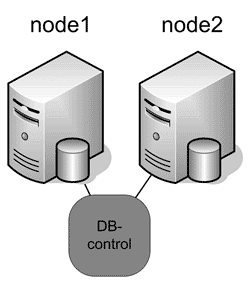
\includegraphics[width=\textwidth]{7/07_03.png}
		\caption{Shared Nothing}
		\label{fig:my_label3}
	\end{subfigure}
	\hfill
	\begin{subfigure}[b]{0.2\textwidth}
		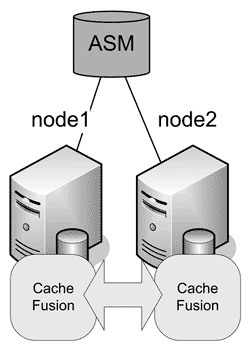
\includegraphics[width=\textwidth]{7/07_04.png}
		\caption{Shared Everything}
		\label{fig:my_label}
	\end{subfigure}
	
	\caption{Кластерные БД}
	\label{fig:my_label4}
\end{figure}


\begin{center}
	\textit{\underline{Распределённые транзакции}}
\end{center}

\href{https://en.wikipedia.org/wiki/Distributed_transaction}{Распределенная транзакция} — это транзакция, затрагивающая несколько ресурсов. Для фиксации распределенной транзакции все участники должны гарантировать, что любое изменение данных будет постоянным. Изменения должны сохраняться даже в случае фатального сбоя системы или других непредвиденных событий. Если хоть один из участников не сможет предоставить такую гарантию, вся транзакция завершится с ошибкой и будет выполнен откат любых изменений данных внутри области транзакции.
